\documentclass[tikz]{standalone}
\usepackage{xcolor}
\usetikzlibrary{3d,calc}


\begin{document}
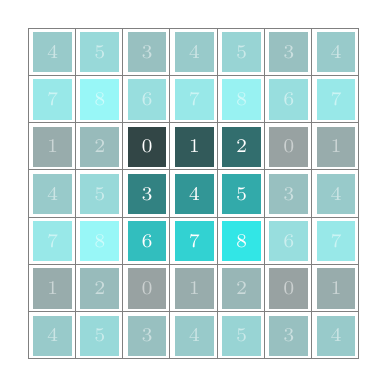
\begin{tikzpicture}[x  = {(1cm,0cm)},
    y  = {(0cm,1cm)},
    z  = {(-.5cm,-.5cm)},
    scale=.6]

  \scriptsize

  \draw [very thin, gray] (0,0) grid (7,7);


  \foreach \pos / \v in {(0,2)/0, (1,2)/1, (2,2)/2, (0,1)/3, (1,1)/4, (2,1)/5, (0,0)/6, (1,0)/7, (2,0)/8} {
      \pgfmathsetmacro{\hue}{70+20*\v} ;
      \draw (2.1,2.05) + \pos node[above right, inner sep=5pt,color=white,fill={rgb,255:red,50;green,\hue;blue,\hue}] {\v} ;
    }

  \foreach \pos / \v in {(0,0)/4,(0,1)/1,(0,2)/7,(0,3)/4,(0,4)/1,(0,5)/7,(0,6)/4} {
      \pgfmathsetmacro{\hue}{70+20*\v} ;
      \draw (0.1,0.05) + \pos node[above right, inner sep=5pt,color=white,opacity=0.5,fill={rgb,255:red,50;green,\hue;blue,\hue}] {\v} ;
    }

  \foreach \pos / \v in {(1,0)/5,(1,1)/2,(1,2)/8,(1,3)/5,(1,4)/2,(1,5)/8,(1,6)/5} {
      \pgfmathsetmacro{\hue}{80+20*\v} ;
      \draw (0.1,0.05) + \pos node[above right, inner sep=5pt,color=white,opacity=0.5,fill={rgb,255:red,50;green,\hue;blue,\hue}] {\v} ;
    }

  \foreach \pos / \v in {(5,0)/3,(5,1)/0,(5,2)/6,(5,3)/3,(5,4)/0,(5,5)/6,(5,6)/3} {
      \pgfmathsetmacro{\hue}{70+20*\v} ;
      \draw (0.1,0.05) + \pos node[above right, inner sep=5pt,color=white,opacity=0.5,fill={rgb,255:red,50;green,\hue;blue,\hue}] {\v} ;
    }

  \foreach \pos / \v in {(6,0)/4,(6,1)/1,(6,2)/7,(6,3)/4,(6,4)/1,(6,5)/7,(6,6)/4} {
      \pgfmathsetmacro{\hue}{70+20*\v} ;
      \draw (0.1,0.05) + \pos node[above right, inner sep=5pt,color=white,opacity=0.5,fill={rgb,255:red,50;green,\hue;blue,\hue}] {\v} ;
    }

  \foreach \pos / \v in {(2,0)/3,(2,1)/0,(3,0)/4,(3,1)/1,(4,0)/5,(4,1)/2} {
      \pgfmathsetmacro{\hue}{70+20*\v} ;
      \draw (0.1,0.05) + \pos node[above right, inner sep=5pt,color=white,opacity=0.5,fill={rgb,255:red,50;green,\hue;blue,\hue}] {\v} ;
    }

  \foreach \pos / \v in {(2,5)/6,(2,6)/3,(3,5)/7,(3,6)/4,(4,5)/8,(4,6)/5} {
      \pgfmathsetmacro{\hue}{70+20*\v} ;
      \draw (0.1,0.05) + \pos node[above right, inner sep=5pt,color=white,opacity=0.5,fill={rgb,255:red,50;green,\hue;blue,\hue}] {\v} ;
    }

\end{tikzpicture}
\end{document}


